\section{The Unified Benchmark}

This section places all three algorithm families on one harness and
establishes the paper's organizing thesis. We report competitive ratios
(mean \(\pm\) 95\% CI) as a function of prediction quality, in three
panels chosen to span the regimes each family was designed for.

\subsection{Design}

The families consume different prediction objects, so we drive each with
its own corruption knob and present them in parallel panels (Section
2.3); the shared harness --- graphs, \(\mathrm{OPT}\), CI methodology,
and the advice-free floor --- is what makes the panels comparable.

\begin{itemize}
\tightlist
\item
  \textbf{Panel A --- clvb\_zipf} (\(n=1000\), 60 trials): heavy-tailed
  offline degrees, the regime where degree predictions carry signal.
\item
  \textbf{Panel B --- left-regular \(d{=}5\)} (\(n=1000\), 60 trials):
  near-homogeneous degrees, where predictions have little to add.
\item
  \textbf{Panel C --- few-types \(r{=}8\)} (\(n=2000\), 50 trials):
  near-perfect-matchable, the calibrated regime for the type-histogram
  test-and-fallback algorithms.
\end{itemize}

For the degree-prediction panels the quality columns are \emph{perfect}
(true degrees), \emph{noisy} (random-flip at strength \(\tfrac12\)),
\emph{adversarial} (order-reversing), and \emph{garbage} (fully random
\(\equiv\) Ranking predictor). For the advice panel the columns are
\(\eta\in\{0,0.3,0.6,1.0\}\) (\emph{perfect / mild / bad / garbage}).
Confidence intervals are tight throughout (\(\pm 0.001\)--\(0.003\)); we
omit them from the prose and report them in Table 1.

\textbf{Table 1} (the three panels, 95\% CI) and \textbf{Figure 1}
(grouped bars) are the section's data. The salient rows:

{ % do not increment counter
\begin{longtable}[]{@{}
  >{\raggedright\arraybackslash}p{(\linewidth - 8\tabcolsep) * \real{0.1579}}
  >{\raggedleft\arraybackslash}p{(\linewidth - 8\tabcolsep) * \real{0.2105}}
  >{\raggedleft\arraybackslash}p{(\linewidth - 8\tabcolsep) * \real{0.2105}}
  >{\raggedleft\arraybackslash}p{(\linewidth - 8\tabcolsep) * \real{0.2105}}
  >{\raggedleft\arraybackslash}p{(\linewidth - 8\tabcolsep) * \real{0.2105}}@{}}
\toprule\noalign{}
\begin{minipage}[b]{\linewidth}\raggedright
\end{minipage} & \begin{minipage}[b]{\linewidth}\raggedleft
perfect
\end{minipage} & \begin{minipage}[b]{\linewidth}\raggedleft
noisy
\end{minipage} & \begin{minipage}[b]{\linewidth}\raggedleft
adversarial
\end{minipage} & \begin{minipage}[b]{\linewidth}\raggedleft
garbage
\end{minipage} \\
\midrule\noalign{}
\endhead
\bottomrule\noalign{}
\endlastfoot
\emph{Panel A --- clvb\_zipf} & & & & \\
Ranking (floor) & 0.948 & --- & --- & --- \\
MinDegree (oracle) & 0.996 & --- & --- & --- \\
MPD & 0.989 & 0.956 & \textbf{0.908} & 0.946 \\
Feldman(MPD) & 0.981 & 0.979 & 0.976 & 0.978 \\
JailletLu(MPD) & 0.977 & 0.976 & 0.974 & 0.975 \\
Feldman / JailletLu (base) & 0.887 / 0.900 & --- & --- & --- \\
\emph{Panel B --- left-regular \(d{=}5\)} & & & & \\
Greedy = Ranking (floor) & 0.890 & --- & --- & --- \\
MinDegree (oracle) & 0.966 & --- & --- & --- \\
MPD & 0.932 & 0.906 & \textbf{0.854} & 0.888 \\
Feldman(MPD) / JailletLu(MPD) & 0.906 / 0.904 & 0.902 / 0.903 & 0.896 /
0.899 & 0.900 / 0.901 \\
Feldman / JailletLu (base) & 0.760 / 0.788 & --- & --- & --- \\
\end{longtable}
}

{ % do not increment counter
\begin{longtable}[]{@{}lrrrr@{}}
\toprule\noalign{}
& perfect & mild & bad & garbage \\
\midrule\noalign{}
\endhead
\bottomrule\noalign{}
\endlastfoot
\emph{Panel C --- few-types \(r{=}8\)} & & & & \\
Ranking (floor) & 0.990 & --- & --- & --- \\
MPD (true degrees) & 0.999 & --- & --- & --- \\
FollowPrediction & 1.000 & 0.832 & 0.679 & \textbf{0.472} \\
TestAndMatch (Choo) & 1.000 & 0.984 & 0.989 & 0.990 \\
TestAndMatch (BEM) & 0.998 & 0.988 & 0.988 & 0.968 \\
Combiner \emph{(benchmark)} & 0.990 & 0.990 & 0.990 & 0.990 \\
\end{longtable}
}

\begin{figure}
\centering
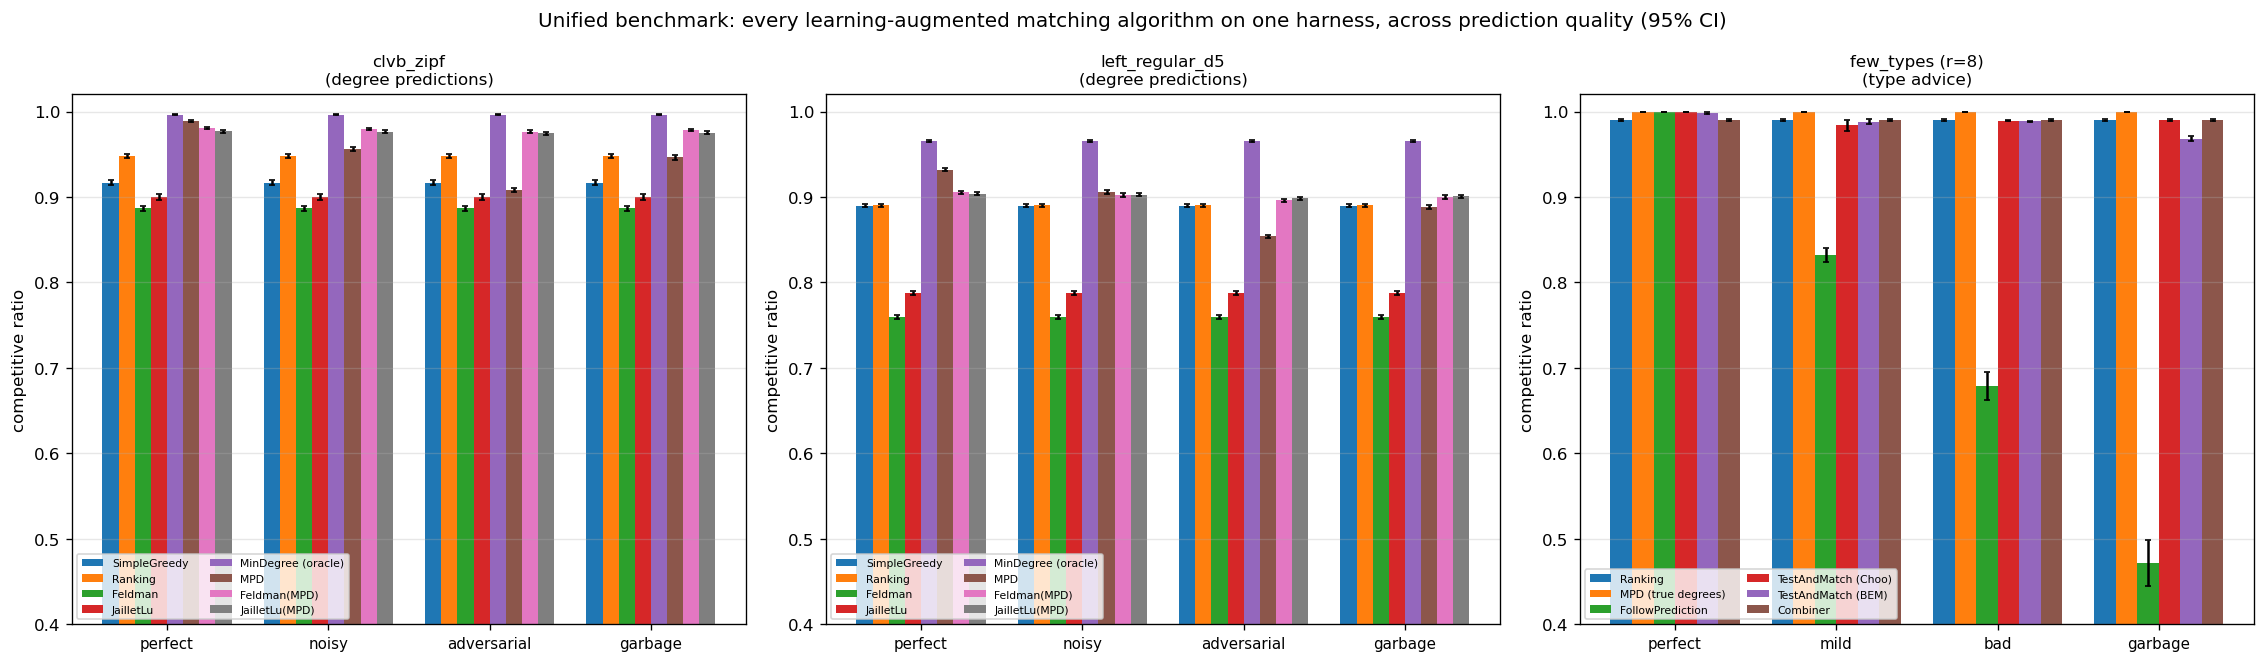
\includegraphics[width=1\linewidth,height=\textheight,keepaspectratio,alt={The unified benchmark (Table 1) as grouped bars: competitive ratio by algorithm and advice quality, one group per panel; the advice-free floor and oracle ceiling bracket every bar.}]{../../results/unified_benchmark.png}
\caption{The unified benchmark (Table 1) as grouped bars: competitive
ratio by algorithm and advice quality, one group per panel; the
advice-free floor and oracle ceiling bracket every bar.}
\end{figure}

\subsection{Four findings}

\textbf{(F1) Robustness is engineered, not free: naive followers crash
below the floor.} Both unguarded prediction-followers dive under the
advice-free Ranking floor once the prediction is adversarial or garbage:
MPD falls to \(0.908 < 0.948\) (Panel A, adversarial) and
\(0.854 < 0.890\) (Panel B), and FollowPrediction collapses to
\(0.472 \ll 0.990\) (Panel C). A practitioner using either
\emph{unguarded} is strictly worse off than using no prediction at all.
Every \emph{robust} algorithm in the tables --- the augmentations,

TestAndMatch, the combiner --- avoids this by construction, not by luck.

\textbf{(F2) Two distinct robustness mechanisms, with different shapes.}
\emph{Structural} robustness (Feldman(MPD), JailletLu(MPD)): a
worst-case-optimal base matching carries the load and the prediction
only breaks ties, so performance is nearly \emph{flat} across quality
--- Feldman(MPD) moves only \(0.981\!\to\!0.976\) from perfect to
adversarial (Panel A). It cannot crash, but it also caps the upside (it
never reaches the \(0.996\) oracle, and sits below MPD's \(0.989\) at
perfect). \emph{Adaptive} robustness (TestAndMatch): test a sublinear
prefix, then commit --- capturing the upside when advice is good (Choo
\(1.000\) at perfect) \emph{and} holding the floor when advice is bad
(\(0.990\) at garbage). On Panel C it is the only algorithm on the upper
envelope at both ends. The two mechanisms trade consistency for
robustness in opposite ways.

\textbf{(F3) The consistency upside is small on average-case inputs; the
spread lives on the bad-advice side.} On few-types the advice-free
Ranking is already \(0.990\) and MPD-with-true-degrees is \(0.999\) ---
under \(0.01\) for \emph{any} advice to add on the good side. Every wide
gap in Panel C (\(1.000\!\to\!0.472\) for FollowPrediction; the
half-wide envelope) is a \emph{downside} gap. This is the thesis in one
panel: learning-augmented matching on typical inputs is robustness
insurance, not a performance lift --- a fact Section 7 prices: safely
capturing an upside this small would take a longer prefix than the
instance itself.

\textbf{(F4) The augmentation rescues structurally weak base
algorithms.} Feldman and Jaillet--Lu are tuned for the worst-case ratio
and are the \emph{weakest} advice-free entries on these average-case
inputs (Panel B: \(0.760\) / \(0.788\), well below Greedy's \(0.890\)).
The MPD augmentation lifts them to \(\approx 0.90\) --- the prediction
does \emph{more} for the worst-case-designed algorithms than for greedy.
This pairing is visible only under a

unified table.

\subsection{Takeaway}

Read together, F1--F4 say that on average-case matching the advice-free
baseline is already near-optimal, unguarded prediction-following is
unsafe, and the value of the sophisticated algorithms is downside
protection delivered by one of two mechanisms. Sections 4--6 sharpen and
stress-test each part --- what governs the (small) loss, what the
adaptive test costs, and whether the picture survives on real graphs,
real traces, and a learned predictor --- and Section 7 proves the wall
is not an artifact but a price: a budget--stakes law that puts the
required test prefix beyond the horizon exactly where the baseline is
strong.
